\documentclass[10pt,notes,compress,aspectratio=169]{beamer}
\usepackage[brazil]{babel}  
\usepackage[utf8]{inputenc}
\usepackage[T1]{fontenc}

\usefonttheme[onlymath]{serif}
\usepackage{beamerthemesplit}
\usetheme{Antibes}

\beamersetuncovermixins{\opaqueness<1->{25}}{\opaqueness<2->{15}}
\setbeamertemplate{itemize items}[triangle]
\setbeamertemplate{enumerate item}{\insertenumlabel)}
\setbeamertemplate{enumerate subitem}{\insertenumlabel-\insertsubenumlabel)}
\setbeamertemplate{caption}[numbered]
\setbeamertemplate{mini frames}{}
\setbeamertemplate{navigation symbols}{}
\setbeamerfont{block title}{size=\scriptsize}
\setbeamerfont{frametitle}{size=\small}
\beamertemplatenavigationsymbolsempty

%%%%%%%%%%%%%%%%%%%%%
% defining frametitle
\setbeamertemplate{frametitle}{%
    \nointerlineskip%
    \begin{beamercolorbox}[wd=\paperwidth,ht=2.5ex,dp=1.0ex]{frametitle}
        \hspace*{2.5ex}\insertframetitle%
    \end{beamercolorbox}%
}
%%%%%%%%%%%%%%%%%%%%%

\newcommand{\hrefcolor}[2]{\textcolor{BlueGreen}{\href{#1}{#2}}}

% Rotating Objects and Captions
\usepackage{hvfloat}

\usepackage{natbib}
\usepackage[brazilian]{cleveref}
\crefname{lstlisting}{lista}{listas}
\Crefname{lstlisting}{Lista}{Listas}

% equation stuff
\usepackage{nicefrac}
\usepackage{cancel}

% table diagonal box
\usepackage{diagbox}
\usepackage{makecell}

% tables
\usepackage{booktabs}

% BEGIN - listings - code in LaTeX
\usepackage{listings}
\renewcommand\lstlistingname{Lista}
\lstset{
  language=octave,
  breaklines=true,
  postbreak=\mbox{$\hookrightarrow$\space},
  basicstyle=\linespread{1}\small\ttfamily,
  %numbers=left,
  numbers=none,
  %frame=lines,
  xleftmargin=0.5cm,
  frame=none,
  framexleftmargin=0.5em,
  framexrightmargin=0.5em,
  %backgroundcolor=\color{light-gray},
  showstringspaces=false,
  upquote=true,
  commentstyle=\color{gray},
  %morecomment=[f][\color{gray}][28]{\#},
  morecomment=[l]{\#\#},
  literate=%
           {á}{{\'a}}1
           {í}{{\'i}}1
           {é}{{\'e}}1
           {ú}{{\'u}}1
           {ó}{{\'o}}1
           {à}{{\`a}}1
           {ã}{{\~a}}1
           {õ}{{\~o}}1
           {â}{{\^a}}1
           {ê}{{\^e}}1
           {ô}{{\^o}}1
           {ç}{{\c{c}}}1
           {Á}{{\'A}}1
           {Í}{{\'I}}1
           {É}{{\'E}}1
           {Ú}{{\'U}}1
           {Ó}{{\'O}}1
           {À}{{\`A}}1
           {Ã}{{\~A}}1
           {Õ}{{\~O}}1
           {Â}{{\^A}}1
           {Ê}{{\^E}}1
           {Ô}{{\^O}}1
           {Ç}{{\c{C}}}1
}
% END - listings

%\usepackage{amsthm}
%\newtheorem{theorem}{Theorem}
%\newtheorem{corollary}{Corollary}
%\newtheorem{lemma}{Lemma}
\newtheorem{proposition}{Proposition}
\newtheorem{axiom}{Axiom}
%\newtheorem{example}{Example}
%\newtheorem{definition}{Definition}
\newtheorem{remark}{Remark}

\usepackage{etoolbox}
\patchcmd{\theorem}{Theorem}{Teorema}{}{}
\patchcmd{\corollary}{Corollary}{Corolário}{}{}
\patchcmd{\lemma}{Lemma}{Lema}{}{}
\patchcmd{\proposition}{Proposition}{Proposição}{}{}
\patchcmd{\axiom}{Axiom}{Axioma}{}{}
\patchcmd{\example}{Example}{Exemplo}{}{}
\patchcmd{\definition}{Definition}{Definição}{}{}
\patchcmd{\remark}{Remark}{Observação}{}{}

%\patchcmd{\theorem}{Theorem}{Teorema}{}{}
%\patchcmd{\corollary}{Corollary}{Corolário}{}{}
%\patchcmd{\lemma}{Lemma}{Lema}{}{}
%\patchcmd{\proposition}{Proposition}{Proposição}{}{}
%\patchcmd{\axiom}{Axiom}{Axioma}{}{}
%\patchcmd{\example}{Example}{Exemplo}{}{}
%\patchcmd{\definition}{Definition}{Definição}{}{}
%\patchcmd{\remark}{Remark}{Observação}{}{}

%\newtheorem{exercise}[theorem]{Exercício}


\newcommand*{\theorembreak}{\usebeamertemplate{theorem end}\framebreak\usebeamertemplate{theorem begin}}
\newcommand*{\proofbreak}{\hfill ...\usebeamertemplate{proof end}\framebreak\usebeamertemplate{proof begin}{\scriptsize\color{gray}continuação...}\\}
\newcommand*{\examplebreak}{\hfill ...\usebeamertemplate{theorem end}\framebreak\usebeamertemplate{theorem begin}{\scriptsize\color{gray}continuação...}\\}
\newcommand*{\exercisebreak}{\hfill ...\usebeamertemplate{theorem end}\framebreak\usebeamertemplate{theorem begin}{\scriptsize\color{gray}continuação...}\\}
\newcommand*{\lemmabreak}{\hfill ...\usebeamertemplate{theorem end}\framebreak\usebeamertemplate{theorem begin}{\scriptsize\color{gray}continuação...}\\}
\newcommand*{\blockbreak}{\hfill ...\usebeamertemplate{block end}\framebreak\usebeamertemplate{block begin}{\scriptsize\color{gray}continuação...}\\}
\newcommand*{\definitionbreak}{\hfill ...\usebeamertemplate{theorem end}\framebreak\usebeamertemplate{theorem begin}{\scriptsize\color{gray}continuação...}\\}

% math symbols

% symbol for independet
\newcommand\independent{\protect\mathpalette{\protect\independenT}{\perp}}
\def\independenT#1#2{\mathrel{\rlap{$#1#2$}\mkern2mu{#1#2}}}
% Real Numbers
\newcommand\RealNumber{{\rm I\!R}}
% Expected value, Variance and Covariance
\newcommand{\E}{\mathrm{E}}
\newcommand{\Var}{\mathrm{Var}}
\newcommand{\Cov}{\mathrm{Cov}}

%%%%%%%%%%%%%%%%%
% math cancel to (down arrow)
\makeatletter
% #1, #2 offset of label   #6 extra width to clear arrowhead
% #3, #4 vector direction  #7 superscript label style
% #5 vector width          #8 superscript label
\def\cantox@vector#1#2#3#4#5#6#7#8{%
  \dimen@.5\p@
  \setbox\z@\vbox{\boxmaxdepth.5\p@
   \hbox{\kern-1.2\p@\kern#1\dimen@$#7{#8}\m@th$}}%
  \ifx\canto@fil\hidewidth  \wd\z@\z@ \else \kern-#6\unitlength \fi
  \ooalign{%
    \canto@fil$\m@th \CancelColor
    \vcenter{\hbox{\dimen@#6\unitlength \kern\dimen@
      \multiply\dimen@#4\divide\dimen@#3 \vrule\@depth\dimen@\@width\z@
      \vector(#3,-#4){#5}%
    }}_{\raise-#2\dimen@\copy\z@\kern-\scriptspace}$%
    \canto@fil \cr
    \hfil \box\@tempboxa \kern\wd\z@ \hfil \cr}}
\def\bcancelto#1#2{\let\canto@vector\cantox@vector\cancelto{#1}{#2}}
\makeatother
%%%%%%%%%%%%%%%%%


%%%%%%%%%%%%%%%%%
% left-right arrow
\makeatletter
\newcommand\xleftrightarrow[2][]{%
  \ext@arrow 9999{\longleftrightarrowfill@}{#1}{#2}}
\newcommand\longleftrightarrowfill@{%
  \arrowfill@\leftarrow\relbar\rightarrow}
\makeatother
%%%%%%%%%%%%%%%%%


%%%%%%%%%%%%%%%%%
% commands to resume enumeration across frames 
\newcounter{sauvegardeenumi}
\newcommand{\asuivre}{\setcounter{sauvegardeenumi}{\theenumi}}
\newcommand{\suite}{\setcounter{enumi}{\thesauvegardeenumi}}
%%%%%%%%%%%%%%%%%

%%%%%%%%%%%%%%%%% underbrase - font size no change
\newcommand*{\KeepStyleUnderBrace}[1]{%
  \mathop{%
    \mathchoice
    {\underbrace{\displaystyle#1}}%
    {\underbrace{\textstyle#1}}%
    {\underbrace{\scriptstyle#1}}%
    {\underbrace{\scriptscriptstyle#1}}%
  }\limits
}
%%%%%%%%%%%%%%%%%

%%%%%%%%%%%%%%%%% math operators
\DeclareMathOperator*{\argmin}{\arg\!\min}
\DeclareMathOperator*{\argmax}{\arg\!\max}
\DeclareMathOperator{\sign}{sign}
\DeclareMathOperator{\Tr}{Tr}
%%%%%%%%%%%%%%%%%


%%%%%%%%%%%%%%%%%
\newenvironment{inlineitemize}{%
 \let\par\relax%
 \def\item{\usebeamertemplate{itemize item}\hspace{1mm}}
 \leavevmode%
}{}

\newenvironment{inlineenumerate}{%
 \let\par\relax%
 \setcounter{enumi}{1}%
 \def\item{\usebeamertemplate{enumerate  item} \stepcounter{enumi}}%
 \leavevmode%
}{%
 \setcounter{enumi}{0}%
}
%%%%%%%%%%%%%%%%%




\title[Processamento de Áudio e Vídeo]{Processamento de Áudio e Vídeo}
\author[Prof. Leonardo Araújo]{Prof. Leonardo Araújo}
\date{}


\begin{document}
\frame{\titlepage}

\frame{\centering 
\includegraphics[width=0.4\textwidth]{images/qrcode-aev.pdf} \\ \url{https://sites.google.com/site/leolca/teaching/multimedia-signal-processing}}

\frame[allowframebreaks]{\begin{footnotesize}\tableofcontents\end{footnotesize}}

% introdução
\section{Introdução}

\begin{frame}%[allowframebreaks]
  \frametitle{Processamento de Áudio e Vídeo}
 
  \begin{itemize}
  \item Compressão
  \item Com/Sem perdas
  \item mp3, jpeg, mpeg, flac, zip, gif, png, etc
  \item sinais de áudio, fala, imagens e vídeo
  \item qualidade, taxa de compressão, custo
  \end{itemize} 

\end{frame}
\note{
  \begin{itemize}
  \item O conceito de compressão surge naturalmente quando estamos lidando com comunicação.
  \item Compressão de dados é o processo de converter dados provenientes de uma fonte em
  outros dados com menor tamanho.
  \item Armazenamento e transmissão (no fundo, ambos são formas de comunicação). 
    \begin{itemize}
    \item linha telefônica analógica
    \item comunicação digital através desta linha telefônica analógica
    \item link de comunicação de rádio entre a sonda espacial Galileu orbitando Júpiter e a Terra
    \item armazenamento e reprodução de áudio ou vídeo (ou dados) em um CD, DVD ou disco rígido
    \item reprodução celular em que a informação sobre as células é contida no DNA
    \end{itemize}
  \end{itemize}
}
\note{
  Métodos de compressão sem perda (alguns são vistos na disciplina Teoria da Informação)
  possuem como limite a entropia. Reconstrução exata da mensagem produzida pela fonte.
  Remover redundância.

  \vspace{2ex}
  Métodos de compressão com perda utilizam-se do fato de que muita informação pode ser 
  perdida sem ser percebida ou aceita-se uma distorção do sinal em prol de uma maior compressão.
}
\note{
\begin{itemize}
\item Áudio, fala, imagens e vídeo são originalmente sinais analógicos.
\item Conversão em sinais digitais: amostragem, quantização, codificação.
\end{itemize}
}
\note{
A qualidade da compressão pode ser uma medida objetiva ou subjetiva.
Na maioria das vezes, iremos realizar medidas objetivas pois realizar
testes subjetivos é muito dispendioso. Podemos escolher medidas objetivas 
que sejam bem correlacionadas com medidas subjetivas.

O custo de compressão e descompressão podem, em geral, serem diferentes.
Descompressão deve ser privilegiada pois é realizada diversas vezes e geralmente
por terminais com menor poder computacional.
}


\begin{frame}%[allowframebreaks]
  \frametitle{Imagem digital}

  \begin{figure}[h]
  \centering
  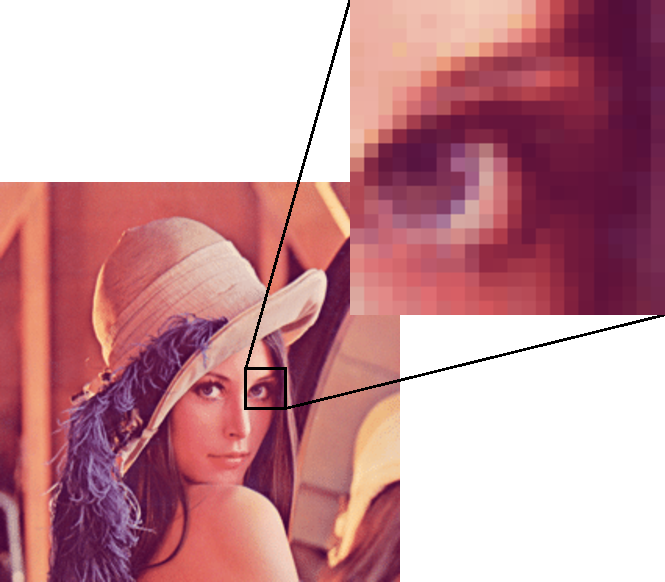
\includegraphics[width=0.5\textwidth]{images/lenaeye.pdf}
  \caption{Lena - detalhe.}\label{fig-lena-detalhe}
  \end{figure}

\end{frame} 

\begin{frame}%[allowframebreaks]
  \frametitle{Espaço necessário para armazenar uma foto}
  \begin{itemize}
  \item câmera 10 Mpixel
  \item 3 bytes por pixel (RGB)
  \item cada foto requer 30 Mbyte
  \item um cartão de memória de 2 Gbytes é capaz de armazenar 66 fotos
  \end{itemize}
\end{frame}

\begin{frame}%[allowframebreaks]
  \frametitle{Espaço necessário para armazenar um vídeo}
  \begin{itemize}
  \item 480 x 720, 30 fps
  \item 345.600 pixels por frame
  \item RGB 3 bytes por pixel
  \item 1.036.800 byte, aprox. 1 Mbyte por frame
  \item 30 frames requerem 31.104.000 bytes, aprox. 31 Mbyte por segundo
  \item um CD de 650 Mbytes é capaz de armazenar apenas 21 segundos de vídeo
  e um DVD de 4.7 GB apenas 155 segundos de vídeo.
  \end{itemize}
\end{frame}


\begin{frame}%[allowframebreaks]
  \frametitle{Dilema de compressão}
  Quando devemos parar a busca por uma \textbf{melhor} compressão?

  \vspace{1cm}
  melhor:
  \begin{itemize}
  \item menor tamanho da representação digital resultante
  \item eficiência computacional (compressão e/ou descompressão)
  \item simplicidade do algoritmo
  \end{itemize}

  \vspace{1cm}
  Qual é o limite de compressão para um determinado dado?

\end{frame} 
\note{
Modificar um algoritmo para melhorar a taxa de compressão em 1\% pode
acarretar um aumento de 10\% no tempo de execução do algoritmo e
ainda mais sobre a complexidade do programa.
}
\note{
Conjecturas\footnote{Uma conjectura é uma proposição que não é provada, mas acredita-se que seja verdadeira e não foi mostrado o contrário.}.
\vspace{2ex}

  \begin{itemize}
  \item Compressão de dados pode ser interpretada como o processo de remover complexidades (redundâncias)
  desnecessárias na informação, e desta forma, maximizando a simplicidade enquanto preserva o máximo
  possível do poder discricionário dos dados.
  \item Todo tipo de computação e racionalização formal pode ser compreendida como compressão
  de informação através do processo de identificar padrões, busca e unificação
  das instâncias destes padrões.
  \end{itemize}

}


\begin{frame}[allowframebreaks]
  \frametitle{Termos}
  \begin{description}
  \item[compressor ou codificador] é o programa que comprime os dados crus na entrada e cria uma saída de dados
  comprimida (com baixa redundância).
  \item[decompressor ou decodificador] converte os dados na direção oposta.
  \item[fluxo] é o dado a ser comprimido, armazenado como um arquivo ou transmitido.
  \item[dado não-codificado, cru, ou original] é o fluxo de dados da entrada.
  \item[dado codificado ou comprimido] é o fluxo de saída.
  \item[método de compressão não-adaptativo] é rígido e não modifica sua operação ou seus parâmetros em resposta
  aos dados em particular que estão sendo comprimidos.
  \item[método adaptativo] analisa os dados crus e modifica sua operação e/ou parâmetros de acordo com os dados em mãos.
  \item[método semi-adaptativo] utiliza 2 passagens aonde, na primeira, realiza a leitura dos dados e
  contabiliza estatísticas dos dados a serem comprimidos; na segunda passagem, realiza de fato a compressão
  utilizados parâmetros determinados na primeira varredura.
  \item[método localmente adaptativo] se adapta às condições locais do fluxo de dados e varia à medida que
  move ao longo dos dados.
  \item[compressão com perdas/sem perdas] : Para atingirem maior compressão, os métodos de compressão com perda
  perdem informação. Os métodos de compressão sem perda não admitem perder informação alguma.
  \item[Compressão em cascata] ocorre quando diferentes métodos de compressão são utilizados um em seguida do outro.
  \item[Compressçao perceptiva] ocorre quando apenas a informação imperceptível pelos nosso sentidos é removida.
  \item[Compressão simétrica] é o caso em que o compressor e descompressor utilizam basicamente o mesmo algoritmo,
  porém em direções opostas.
  \item[Complacente] é o codificador/decodificador que gera/lê de forma correta um fluxo de dados (Qualquer pessoa
  é livre para implementar seu próprio algoritmo).
  \item[Universal] é o método de compressão de dados que não depende da estatística dos dados.
  \item[Razão de Compresão] $=$ tamanho do dado de saída / tamanho do dado de entrada.
  \item[Fator de Compressão] $=$ tamanho do dado de entrada / tamanho do dado de saída $=$ (razão de compressão)$^{-1}$.
  \item[Ganho de Compressão] $= 100 \log_e $ (tamanho de referência / tamanho comprimido), aonde o tamanho de referência é o tamanho dos dados de entrada ou o tamanho do dado de saída comprimido por algum algoritmo padrão.
  \item[Erro médio quadrático (MSE) e relação sinal ruído de sinal (PSNR)] são utilizados para medir a distorção causada por uma compressão com perdas.
  \end{description}
\end{frame} 


\begin{frame}%[allowframebreaks]
  \frametitle{Termos}
  \begin{figure}[h]
  \centering
  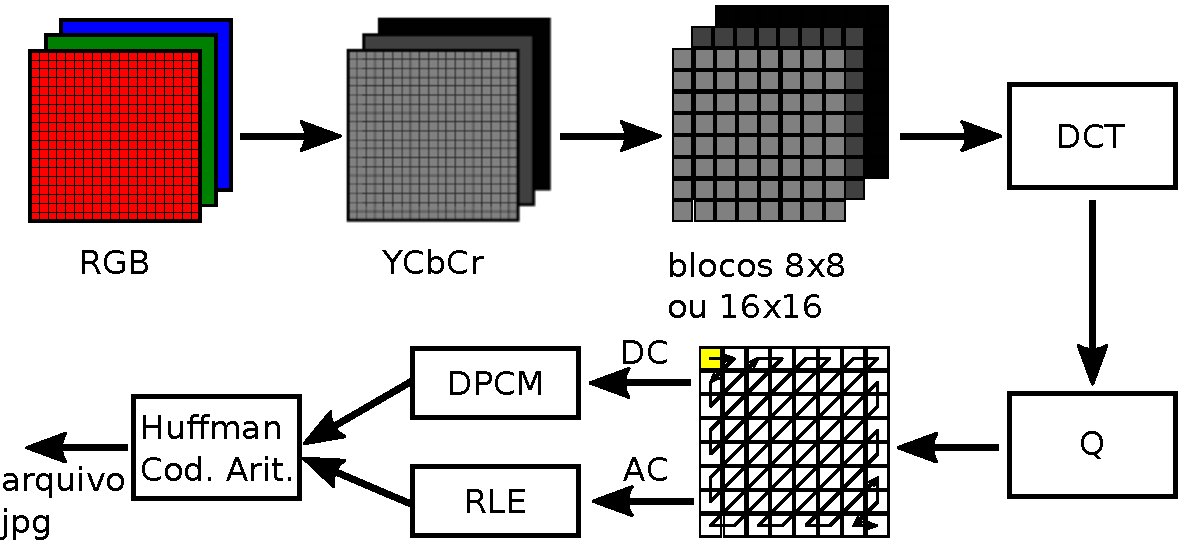
\includegraphics[width=0.8\textwidth]{images/jpegstd.pdf}
  \caption{Esquema de compressão JPEG.}\label{fig-jpegstd}
  \end{figure}
\end{frame} 

\begin{frame}%[allowframebreaks]
  \frametitle{Slides- introdução ao GNU Octave}
  \centering
  
\includegraphics[width=0.4\textwidth]{images/qrcode-octave-intro.pdf}

  \url{https://drive.google.com/open?id=1ew5fl9v_OIybsy3KdEgIvohLTcuwuru_}
\end{frame} 

\begin{frame}%[allowframebreaks]
  \frametitle{Notebook - introdução}
  \centering
  
\includegraphics[width=0.4\textwidth]{images/qrcode-jupyter-intro.pdf}

  \url{https://nbviewer.jupyter.org/github/leolca/notebooks/blob/master/aev/introducao.ipynb}
\end{frame} 

\begin{frame}%[allowframebreaks]
  \frametitle{Notebook - imagem colorida}
  \centering
  
\includegraphics[width=0.4\textwidth]{images/qrcode-jupyter-im-color.pdf}

  \url{https://nbviewer.jupyter.org/github/leolca/notebooks/blob/master/aev/introdocao_imagem_colorida.ipynb}
\end{frame} 



\section{Tecnicas Básicas de Compressão}

\begin{frame}%[allowframebreaks]
  \frametitle{Leitura}
  \centering
  
\includegraphics[width=0.4\textwidth]{images/qrcode-book-salomon.pdf}

  David Salomon, Giovanni Motta - \textit{Handbook of Data Compression}, 2010 \\ 
  \url{https://books.google.com.br/books?id=LHCY4VbiFqAC}\\
  Introduction, Basic Techniques \citep{salomon2010}
\end{frame} 

\subsection{RLE}
\begin{frame}%[allowframebreaks]
  \frametitle{Compressão RLE}
   
  Exemplo:

  string: `2. all is too well'

  codificação: `2. a@2l is t@2o we@2l'

  \vspace{1cm}
  Método MNP5 era utilizado nos modems antigos.

\end{frame}
\note{
MNP : Microcom Networking Protocol

"The MNP5 method is a two-stage process that starts with run-length encoding, followed by adaptive frequency encoding."
\citep{salomon2000}

"With MNP 5, the data received from the computer are first compressed with a simple algorithm, and then passed into the MNP 4 packetizing system for transmission. On best-case data the system offered about 2:1 compression, but in general terms about 1.6:1 was typical, at least on text. As a result a 2400 bit/s modem would appear to transfer text at ~4000 bit/s, even though the modem was still running at the same 600 baud * 4 bits per symbol rate.

This dramatic increase in throughput allowed Microcom modems to remain somewhat competitive with models from other companies that were otherwise nominally much faster. For instance, Microcom generally produced 1200 and 2400 bit/s modems using commodity parts, while companies like USRobotics and Telebit offered models with speeds up to 19200 bit/s."
(\url{https://en.wikipedia.org/wiki/Microcom_Networking_Protocol})
}


\begin{frame}%[allowframebreaks]
  \frametitle{Compressão RLE}
 
  Exemplo: uma imagem em tons de cinza com 8-bit de profundidade começa com os seguintes valores

  12, 12, 12, 12, 12, 12, 12, 12, 12, 35, 76, 112, 67, 87, 87, 87, 5, 5, 5, 5, 5, 5, 1, ...

  será comprimida como  \framebox{9},12,35,76,112,67,\framebox{3},87,\framebox{6},5,1, ...

  \vspace{1cm}
  Se utilizarmos como \textit{flag} o valor 255, então a sequência acima será expressa por

  255, 9, 12, 35, 76, 112, 67, 255, 3, 87, 255, 6, 5, 1, ...

  \vspace{1cm}
  grupos de 8

  \framebox{10000010},9,12,35,76,112,67,3,87,\framebox{100...},6,5,1, ...

\end{frame} 

\begin{frame}%[allowframebreaks]
  \frametitle{Exemplo RLE - GNU Octave}
  \centering
  
\includegraphics[width=0.4\textwidth]{images/qrcode-jupyter-rle.pdf}

  \url{https://nbviewer.jupyter.org/github/leolca/notebooks/blob/master/aev/rle_mario.ipynb}
\end{frame} 


\begin{frame}%[allowframebreaks]
  \frametitle{Move-to-Front Coding}
  Consideramos o alfabeto de símbolos $\mathcal{A}$ como uma lista 
  onde os símbolos mais frequentes estarão dispostos no início da lista.

  O método é localmente adaptativo, já que ele se adapta à frequência dos
  símbolos em cada região do fluxo de dados.
\end{frame} 


\begin{frame}%[allowframebreaks]
  \frametitle{Move-to-Front Coding - Exemplo \citep{salomon2010}}

   Exemplo:
   entrada a ser codificada: \textbf{abcddcbamnopponm}

  \begin{columns}[c]
  \column{.4\textwidth}
  C = (0, 1, 2, 3, 0, 1, 2, 3, 4, 5, 6, 7, 0, 1, 2, 3) \\
  -- utilizando move-to-front\\
  \vspace{1cm}
  C' = (0, 1, 2, 3, 3, 2, 1, 0, 4, 5, 6, 7, 7, 6, 5, 4) \\
  -- sem utilizar move-to-front 
  \column{.6\textwidth}
     \vspace{-0.2cm}
     \begin{figure}[h!]
     \centering
     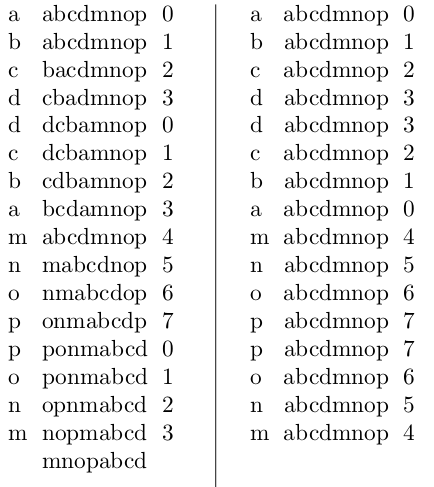
\includegraphics[width=0.7\textwidth]{images/move_to_front_coding.png}
     %\caption{}
     \label{fig:move_to_front_coding}
     \end{figure}
  \end{columns}

\end{frame} 

\begin{frame}%[allowframebreaks]
  \frametitle{Move-to-Front Coding - Exemplo \citep{salomon2010}}
  \begin{columns}[c]
  \column{.4\textwidth}
  O resultado $C$ obtido pelo move-to-front é tal que, na média, os valores
  em $C$ são pequenos (os valores no início do dicionário são os mais prováveis).
  Isto faz com que a saída seja propícia para ser codificada através da codificação
  de Huffman ou codificação aritmética.
  \column{.4\textwidth}
     \begin{figure}[h!]
     \centering
     \includegraphics[width=0.65\textwidth]{/home/leoca/ee/ufsj/2012_01/audio_video/aulas/images/variable_sized_codes.png}
     \caption{Exemplo de código de tamanho variável.}
     \label{fig:variable_sized_codes}
     \end{figure}
  \end{columns}

\end{frame}


\begin{frame}%[allowframebreaks]
  \frametitle{Move-to-Front Coding}
  Variações:
  \begin{enumerate}
  \item Move-ahead-k: O elemento do alfabeto A que corresponde ao símbolo corrente será deslocado k posições para cima na lista ao
          invés de ir para o topo da lista.
  \item Wait-c-and-move: O elemento do alfabeto A será deslocado para o início da lista apenas após aparecer c vezes durante a
          codificação. 
  item Wait-c-and-ahead-k: Um combinação das duas variantes anteriores.
  \end{enumerate}

\end{frame} 

\begin{frame}%[allowframebreaks]
  \frametitle{Exemplo Move-to-Front - GNU Octave}
  \centering
  
\includegraphics[width=0.4\textwidth]{images/qrcode-jupyter-m2f.pdf}

  \url{https://nbviewer.jupyter.org/github/leolca/notebooks/blob/master/aev/move-to-front.ipynb}
\end{frame} 






\bibliographystyle{apalike}
\bibliography{bibliografia}
\label{bibliografia}

\end{document}

